\documentclass[12pt, a4paper]{article}

% Standard packages for economics papers
\usepackage[utf8]{inputenc}
\usepackage[T1]{fontenc}
\usepackage{geometry}
\geometry{a4paper, margin=1in}
\usepackage{setspace}
\onehalfspacing % Common for readability; use \doublespacing if submitting for review
\usepackage{amsmath, amssymb, amsthm}
\usepackage{graphicx}
\usepackage{booktabs}  % Creates beautiful top/mid/bottom rules instead of ugly grids
\usepackage{multirow}  % Allows the p0 values to span across the T rows seamlessly
\usepackage{rotating}  % Allows for sideways tables (sidewaystable)
\usepackage{caption}
\usepackage{subcaption}
\usepackage[colorlinks=true, linkcolor=blue, citecolor=blue, urlcolor=blue]{hyperref}

% Make it fit 10 pages
\usepackage{fullpage} % Slightly reduces standard 1-inch margins
\linespread{0.98} % Reduces line spacing by a virtually unnoticeable 2%
\setlength{\parskip}{0pt plus 1pt} % Minimizes spacing between paragraphs
\setlength{\parsep}{0pt} % Reduces internal paragraph spacing
\usepackage{enumitem}
\let\oldbibliography\bibliography
\renewcommand{\bibliography}[1]{
  \setlength{\itemsep}{0pt} % Removes spacing between references
  \setlength{\parsep}{0pt}
  \oldbibliography{#1}
}
\usepackage{titlesec}
\titlespacing*{\section}{0pt}{12pt plus 2pt minus 2pt}{6pt plus 2pt}
\titlespacing*{\subsection}{0pt}{10pt plus 2pt minus 2pt}{4pt plus 2pt}
\setlength{\textfloatsep}{10pt plus 2pt minus 4pt} % Space between top/bottom floats and text
\setlength{\floatsep}{8pt plus 2pt minus 2pt} % Space between two floats
\setlength{\intextsep}{8pt plus 2pt minus 2pt} % Space for in-text floats



% Package to format assumptions
\usepackage{amsthm}
\usepackage{thmtools}
\declaretheoremstyle[
  headfont=\bfseries, 
  bodyfont=\normalfont, % keeps text upright, not italic
  spaceabove=6pt, 
  spacebelow=6pt
]{assumptionstyle}
\declaretheorem[style=assumptionstyle, name=Assumption]{assumption}
\declaretheorem[name=Theorem]{theorem}
\declaretheorem[name=Lemma]{lemma}
\declaretheorem[name=Definition]{definition}

% BibLaTeX setup for Zotero Better BibLaTeX
\usepackage[
  style=authoryear, 
  backend=biber, 
  natbib=true, 
  maxcitenames=2,
  isbn=false,   % Hides ISSN and ISBN fields
  doi=false,    % Hides DOI fields
  url=false,    % Hides URL fields
  urldate=comp, % Hides "visited on" date fields
  eprint=false  % Hides Google Books, JSTOR, arXiv, and other eprint IDs
]{biblatex}
\addbibresource{DML_Policy_Project.bib}

% Option A: Global fix for biblatex font size (Put this in the preamble)
\renewcommand*{\bibfont}{\footnotesize} 

% Change formatting to fit policy report style:
\renewcommand{\abstractname}{Executive Summary}

% Title and Author Information
\title{Urban Policies to Combat Climate Change: \\ Assessing the Impact of Congestion Pricing and Low-Emission Zones using Machine Learning Techniques}
\author{
    Ferdinand Loser\thanks{Ludwig-Maximilian University of Munich, \href{mailto:ferdinand.loser@campus.lmu.de}{ferdinand.loser@campus.lmu.de} \\ Replication files are available in the \href{https://github.com/FerdinandLos/machine-learning-policy}{GitHub repository} for this project. The coding files are also uploaded on Moodle.}
}
\date{\today \\ \vspace{0.5cm} Course: \textit{Machine Learning in Econometrics} \\ Prof. Daniel Wilhelm \\ \vspace{0.5cm} Ludwig-Maximilian University of Munich, M. Sc. Economics Program}

\begin{document}

\maketitle
\thispagestyle{empty}

\begin{abstract}
\noindent
This report evaluates the effectiveness of Congestion Pricing (CP) and Low-Emission Zones (LEZs) on urban transport $CO_2$ emissions across 183 cities from 2008 to 2024 using a Double Machine Learning framework. Applying LASSO orthogonalization alongside Augmented Inverse Propensity Weighting (AIPW) and Causal Forest algorithms, the analysis reveals that CP yields a substantial 27\% to 33\% reduction in emissions, significantly outperforming the 10\% to 19\% reduction driven by LEZs. Furthermore, k-means clustering demonstrates that climate policy efficacy depends on urban structural typologies: CP is highly effective in \textit{Sprawling Regional Hubs} where LEZs fail, while both policies are viable and effective in \textit{Dense Metropolises}. Finally, the lack of common support between treatment and control group prevents the reliable estimation of simultaneous synergetic effects.
\end{abstract}

\clearpage % Moves to the second page
\pagenumbering{arabic} 

\section{Introduction}

\label{sec:introduction}

Discussions about global warming have been highly prevalent in public discourse, especially in the past 10 to 15 years. Many policies have been implemented, and even more have been proposed and advocated for. Some are to be decided on the supranational level, e.g., the EU's climate certificate trading, some on the national level, e.g., electric vehicle subsidies, but many can also be implemented on the regional or even municipal level. Especially when it comes to reducing transport $CO_2$ emissions, many decisions fall under the authority of the municipal government, be it how road infrastructure is designed, what speed limits are set, or further driving regulations. This report estimates the effectiveness in reducing transport carbon emissions of two such regulatory policies:

\begin{definition}
\textbf{Congestion Pricing (CP): } Surcharges are implemented in certain areas of a city for cars that enter from outside.
\end{definition}
\begin{definition}
\textbf{Low-Emission Zones (LEZ): } Certain vehicles (older diesel or petrol engines) are banned in certain areas of a city.
\end{definition}
I study these two policies in a large panel dataset of 183 cities from 2008 to 2024, focusing especially on three core research questions:

 \textbf{Research Question 1. } Were the policies effective in reducing emissions?

\textbf{Research Question 2. } Which type of cities benefit the most/least from the policies?

\textbf{Research Question 3. } Does implementation of both policies simultaneously produce greater emission reductions than what would have been expected from the sum of the individual effects of implementing either policy alone?

Using the Double Machine Learning framework with LASSO first stage estimation and a comparison of AIPW and Causal Forest for the second stage, my results show that both policies were effective in reducing carbon emissions, yet Congestion Pricing is found to have a stronger impact, decreasing transport $CO_2$ emissions by around 28\% to 32\% whereas LEZs only lead to a reduction of 10\% to 18\%. Evidence is found for a stronger impact of CP in more \textit{Sprawling Regional Hubs}, cities that have a rather small population, large land area, and a high share of petrol vehicles. On the other hand, LEZs are determined to be ineffective in this city type, but beneficial for the type \textit{Dense Metropolis}, i.e. dense, highly populated cities with a higher share of green party voters, and electric and diesel cars. Synergy effects of implementing both policies simultaneously cannot reliably be determined as the group of cities that implemented these policies differs too strongly from cities in the control group.

The remainder of the report is structured as follows. Section~\ref{sec:emp_strategy} introduces the empirical strategy and the identification assumptions underlying the analysis. Section~\ref{sec:proposed_estimator} outlines the proposed estimation framework, while Section~\ref{sec:theoretical_properties} gives the proof of Neyman Orthogonality. Section~\ref{sec:data_preparation} describes the transformation of the empirical dataset and the clustering procedure used to distinguish city types. Section~\ref{sec:results} presents the main empirical findings, Section~\ref{sec:sensitivity_analysis} evaluates robustness and sensitivity checks, and Section~\ref{sec:conclusion} provides an interpretation of the results and their policy implications.

\section{Empirical Strategy and Identification}
\label{sec:emp_strategy}

The target parameters of this study are the Average Treatment Effect on the Treated (ATT) and the Group Average Treatment Effect on the Treated (GATT). The ATT is chosen over the general Average Treatment Effect (ATE) as this report aims to address the question of how efficient these policies were in the cities that really implemented them, not the hypothetical case where all cities are forced to implement the policies.

The global ATT measures the average impact of a specific policy regime across all cities that actually implemented it, evaluated against the baseline of no policy ($d=0$). It is defined as:

\begin{equation}
    \tau_{ATT, d} = \mathbb{E}[Y_{it}(d) - Y_{it}(0) \mid D_{it} = d]
\end{equation}

In this setting, treatment is not binary but has three states: CP ($d=1$), LEZ ($d=2$), and their synergy CP $\times$ LEZ ($d=3$).  

To address research question 2 regarding spatial heterogeneity, the GATT isolates this treatment effect within the specific structural typologies $G_i$. The two clusters $G_i \in \{0, 1\}$ are constructed using k-means clustering on $X_i = [X_{i}^{invariant}, \bar{X}_{i}^{pre-treatment}]$, both time-invariant factors like geographical features as well as pre-treatment averages of covariates, so called Mundlak devices (see Section~\ref{sec:data_preparation}). The GATT for each cluster is therefore defined as:

\begin{equation}
    \tau_{GATT, d}(g) = \mathbb{E}[Y_{it}(d) - Y_{it}(0) \mid D_{it} = d, G_i = g] \quad \text{for } g \in \{0, 1\}
\end{equation}

For the ATT and GATT to be identified correctly, three assumptions are required.

\begin{assumption}\label{as:cond_independence}
\textbf{Conditional Independence/Ignorability: } $(Y(d), Y(0)) \perp\!\!\!\perp D \mid X_i$. Conditional on the Mundlak device and baseline geography, treatment assignment is independent of potential outcomes. I.e., variables of $X_i$ encompass all relevant factors that determine whether a city implements policy $d$ \citep[Ch. 5]{CausalMLBookAppliedCausal}.
\end{assumption}

\begin{assumption}\label{as:overlap}
\textbf{Weak Overlap: } $P(D=1 \mid X) < 1$. Policy implementation cannot be perfectly predicted by the pre-treatment covariates $X_i$. I.e., every treated city has a similar untreated counterpart \citep[Ch. 5]{CausalMLBookAppliedCausal}.
\end{assumption}

\begin{assumption}\label{as:sutva}
\textbf{SUTVA: } The potential outcomes of city $i$ are unaffected by the treatment status of city $j$ (no spatial spillovers) \citep[Ch. 2]{CausalMLBookAppliedCausal}.
\end{assumption}

\section{Proposed Estimator}
\label{sec:proposed_estimator}

To estimate the (G)ATT, I employ two different double machine learning approaches: Augmented Inverse Propensity Weighting (AIPW) and Causal Forest, estimating the treatment effects in two stages:

\textbf{Stage 1 (Orthogonalization): } The algorithm first uses LASSO to estimate two "nuisance" functions using cross-fitting with 5 folds, whereby the hyperparameters $\alpha$ and $C$ are determined once outside the cross-fitting to save computation time. The two nuisance functions are as such:

\begin{itemize}
    \item The propensity score: $p(W_{it}) = \mathbb{E}[D_{it} \mid W_{it}]$ is estimated via a logistic regression with L1 Lasso penalty. Then the Treatment Residual: $\tilde{D}_{it} = D_{it} - \hat{p}(W_{it})$ is calculated as the leftover residual of the true treatment $D_{it}$ minus the predicted propensity score $\hat{p}(W_{it})$ for each city-time observation, representing how much of the variable could not be explained by the regression.
    \item The expected outcome: $m(W_{it}) = \mathbb{E}[Y_{it} \mid W_{it}]$ is estimated via a linear LASSO regression. Then the Outcome Residual: $\tilde{Y}_{it} = Y_{it} - \hat{m}(W_{it})$ is calculated as the leftover residual of the true outcome $Y_{it}$ minus the predicted outcome $\hat{m}(W_{it})$ for each city-time observation.
\end{itemize}

Both of these LASSO regressions are fit with the whole set $W_{it} = X_{it} + X_i$, both contemporary and time-invariant covariates, whereby the LASSO penalty shrinks down and eliminates covariates to minimize prediction error in a cross-validation setting.\footnote{$W_it$ also omits other variables that are expected to be impacted by or to impact either of the two policies such as e.g. PM2.5 emissions, vehicle engine shares, or records of public announcement of such policies.} This stage is the same for both AIPW and Causal Forest \citep[See][]{chernozhukovDoubleDebiasedMachine2018}. 

\textbf{Stage 2 (ATT/GATT Estimation): } Here AIPW and Causal Forest differ in how they use the DR scores to estimate the treatment effects.

\textit{AIPW} uses the treatment and outcome residuals ($\tilde{D}_{it}$ and $\tilde{Y}_{it}$) to estimate Doubly Robust scores (DR), a pseudo-outcome of how a specific city-year observation should have been based on what the first stage models can explain. The GATT then represents the average of all individual DR scores of treated cities within a cluster, and the ATT the average of all treated cities \citep[See][]{chernozhukovDoubleDebiasedMachine2018}.

\textit{Causal Forest} builds a large set of trees, 200, whereby each tree uses a random subsample of cities. Each tree is very shallow, consisting of only two terminal nodes (leaves), the clusters for dense metropolises and regional hubs. Then, within each leaf, an OLS regression is fitted on the orthogonalized residuals from Stage 1 ($\tilde{Y}_{it}$ and $\tilde{D}_{it}$). Finally, the estimations of all different leaves are averaged for the final GATT estimate (and then the two GATT estimates averaged for the ATT estimate). The shallowness of the tree is beneficial as it makes estimation within each leaf well estimable, as each leaf still contains a large number of treated and untreated cities, which is especially necessary for estimating the synergy effect, which was relatively rarely implemented in the dataset \citep[See][]{wagerEstimationInferenceHeterogeneous2018, atheyGeneralizedRandomForests2019}.

Finally, standard errors are estimated using clustered bootstrapping in order to account for possible serial correlation of error terms within cities \citep[See][]{cameronBootstrapBasedImprovementsInference2008}. The bootstrap procedure is clustered at the city level. For each bootstrap iteration $b \in \{1, \dots, B\}$, a random sample of cities is drawn with replacement from the original dataset. When a city is selected, its entire time-series trajectory (the "block") is pulled into the bootstrap sample, preserving the intra-city temporal autocorrelation matrix.

For each iteration, the full Double Machine Learning pipeline—including the cross-fitted $L_1$-penalized nuisance estimation and the second-stage causal aggregation—is re-estimated. The empirical standard error (SE) for each treatment effect $\hat{\theta}$ is then calculated as the standard deviation of the resulting bootstrap distribution:
\begin{equation}
    \widehat{SE}(\hat{\theta}) = \sqrt{\frac{1}{B-1} \sum_{b=1}^{B} \left( \hat{\theta}_b - \bar{\hat{\theta}} \right)^2}
\end{equation}
where $\bar{\hat{\theta}}$ is the mean of the bootstrap estimates. Following standard practice for large-$N$ machine learning estimators, the bootstrap estimates are assumed to be asymptotically normal. Statistical significance and $p$-values are computed via a normal approximation, utilizing the $z$-statistic $z = \hat{\theta}_{main} / \widehat{SE}(\hat{\theta})$, where $\hat{\theta}_{main}$ is the point estimate from the original, unresampled dataset. For the final results presented in Section \ref{sec:results}, the procedure was executed with $B = 50$ iterations, a number that may be too low to immunize the standard errors from random variation that was chosen due to computational limitations.


\section{Theoretical Properties}
\label{sec:theoretical_properties}

Both AIPW and the Causal Forest circumvent the inherent regularization bias of Lasso (which stems from L1 penalization) by specifying orthogonal second-stage moments. This prevents the transmission of first-stage prediction errors into the final causal estimates. Their confirmation of Neyman orthogonality is demonstrated in the following two proofs \citep[Based on][]{CausalMLBookAppliedCausal}.

\begin{theorem}\label{the:Neyman_orthogonality_pathwise}
\textbf{Neyman Orthogonality: } Let $Z = (Y, D, W)$ denote the full data vector. A score function $\psi(Z; \theta, \eta)$ identifying a causal parameter $\theta$ with nuisance parameters $\eta$ is Neyman orthogonal if the pathwise (Gateaux) derivative of the expected score with respect to the nuisance parameters, evaluated at their true values $\eta_0$, equals zero for all permissible perturbation directions $h$:


$$\partial_r \mathbb{E}[\psi(Z; \theta_0, \eta_0 + r h)] \Big\vert{}_{r = 0} = 0$$


\end{theorem}

Both AIPW and the Causal Forest circumvent the inherent regularization bias of Lasso (which stems from L1 penalization) by specifying orthogonal second-stage moments. This prevents the transmission of first-stage functional prediction errors into the final causal estimates. Their confirmation of Neyman orthogonality is demonstrated in the following two proofs.

\begin{proof}\label{proof:Neyman_orthogonality_aipw}
\textbf{AIPW (Doubly Robust Score for the Treated): }Let the parameter of interest $\theta$ be the expected potential outcome under treatment $\mathbb{E}[Y(1)]$. The true nuisance functions are $\eta_0 = (\mu_{1,0}, p_0)$, where $\mu_{1,0}(W) = \mathbb{E}[Y \mid D=1, W]$ and $p_0(W) = \mathbb{E}[D \mid W]$.

The score function is defined as:


$$\psi(Z; \theta, \eta) = \mu_1(W) + \frac{D}{p(W)}\Big(Y - \mu_1(W)\Big) - \theta$$

Orthogonality with respect to the outcome model $\mu_1(W)$:
We consider a perturbed function $\mu_{1,r}(W) = \mu_{1,0}(W) + r h_\mu(W)$ and differentiate with respect to $r$ at $r=0$. Applying the Law of Iterated Expectations (LIE) conditioning on $W$:


$$\frac{\partial}{\partial r} \mathbb{E}\left[ \mu_{1,0}(W) + r h_\mu(W) + \frac{D}{p_0(W)}\Big(Y - \mu_{1,0}(W) - r h_\mu(W)\Big) - \theta_0 \right] \Bigg\vert{}_{r=0}$$

$$= \mathbb{E}\left[ h_\mu(W) - \frac{D}{p_0(W)}h_\mu(W) \right] = \mathbb{E}_W\left[ h_\mu(W) \left( 1 - \frac{\mathbb{E}[D \mid W]}{p_0(W)} \right) \right] = \mathbb{E}_W\left[ h_\mu(W) ( 1 - 1 ) \right] = 0$$

Orthogonality with respect to the propensity model $p(W)$:
We consider a perturbed function $p_r(W) = p_0(W) + r h_p(W)$ and differentiate with respect to $r$ at $r=0$. Again, applying the LIE:


$$\frac{\partial}{\partial r} \mathbb{E}\left[ \mu_{1,0}(W) + \frac{D}{p_0(W) + r h_p(W)}\Big(Y - \mu_{1,0}(W)\Big) - \theta_0 \right] \Bigg\vert{}_{r=0}$$

$$= \mathbb{E}\left[ -\frac{D \cdot h_p(W)}{p_0(W)^2}\Big(Y - \mu_{1,0}(W)\Big) \right] = \mathbb{E}_W\left[ -\frac{h_p(W)}{p_0(W)^2} \underbrace{\mathbb{E}[D(Y - \mu_{1,0}(W)) \mid W]}_{=0} \right] = 0$$


\end{proof}

\begin{proof}\label{proof:Neyman_causal_forest}
\textbf{Causal Forest: } Let the parameter $\theta$ be the average treatment effect. The true nuisance functions are $\eta_0 = (m_0, p_0)$, where $m_0(W) = \mathbb{E}[Y \mid W]$ and $p_0(W) = \mathbb{E}[D \mid W]$.

The score function for the partialled-out regression is:


$$\psi(Z; \theta, \eta) = \Big(Y - m(W) - \theta(D - p(W))\Big)\Big(D - p(W)\Big)$$

Orthogonality with respect to the marginal outcome model $m(W)$:
Consider the perturbation $m_r(W) = m_0(W) + r h_m(W)$. Evaluating the derivative at $r=0$ and applying the LIE:


$$\frac{\partial}{\partial r} \mathbb{E}\left[ \Big(Y - (m_0(W) + r h_m(W)) - \theta_0(D - p_0(W))\Big)\Big(D - p_0(W)\Big) \right] \Bigg\vert{}_{r=0}$$

$$= \mathbb{E}\left[ -h_m(W)(D - p_0(W)) \right] = \mathbb{E}_W\left[ -h_m(W) \underbrace{\mathbb{E}[D - p_0(W) \mid W]}_{=0} \right] = 0$$

Orthogonality with respect to the propensity model $p(W)$:
Consider the perturbation $p_r(W) = p_0(W) + r h_p(W)$. Applying the product rule for the derivative with respect to $r$ at $r=0$:


$$\frac{\partial}{\partial r} \mathbb{E}\left[ \Big(Y - m_0(W) - \theta_0(D - (p_0(W) + r h_p(W)))\Big)\Big(D - (p_0(W) + r h_p(W))\Big) \right] \Bigg\vert{}_{r=0}$$

$$= \mathbb{E}\left[ \Big(\theta_0 h_p(W)\Big)\Big(D - p_0(W)\Big) + \Big(Y - m_0(W) - \theta_0(D - p_0(W))\Big)\Big(-h_p(W)\Big) \right]$$

$$= \mathbb{E}\left[ h_p(W) \Big( 2\theta_0(D - p_0(W)) - (Y - m_0(W)) \Big) \right]$$

$$= \mathbb{E}_W\left[ h_p(W) \Big( 2\theta_0 \underbrace{\mathbb{E}[D - p_0(W) \mid W]}_{=0} - \underbrace{\mathbb{E}[Y - m_0(W) \mid W]}_{=0} \Big) \right] = 0$$


\end{proof}

\section{Data Preparation}
\label{sec:data_preparation}

The raw panel dataset, consisting of 51 variables for 183 cities in the time frame from 2008 to 2024, has to be adjusted for a valid estimation via double machine learning. First, minor adjustments are made by changing the categorical variable on the latitude zone into separate dummies as well as log-transforming variables that have highly skewed distributions and/or where it is economically meaningful to do so.\footnote{Log-transformed variables are: Total $CO_2$ Emissions, Population, Population Density, GDP per capita, Land Area, Electricity Price, and Fuel Price.}

For accurate estimation in a panel setting, time-invariant traits have to be controlled for. For this purpose, the dataset already includes some time-invariant covariates $X^{geographic}_i$ depicting geographic features. Additionally, I transform all time-, non-dummy features into time-invariant Mundlak devices $\bar X^{pre}_i$ by taking the within-city average over all periods before the implementation of one of the two policies \citep[See][]{mundlakPoolingTimeSeries1978}. This limitation on pre-periods ensures that potential side-effects of the policies are not altering the averages. One variable that didn't change for any city in any pre-period is dropped: a dummy for signing a national climate pact. Additonally, I add year dummies in order to account for time fixed effects.

\subsection*{K-means clustering}
\label{sec:cluster}

In the next step, I utilize the whole set of time-invariant covariates $X_i$ with the exception of latitude dummies in order to run k-means clustering to determine a good split of the city features into two types \citep[See][Ch. 12.4.1]{jamesIntroductionStatisticalLearning2023}. The benefit of using clusters instead of raw covariates for the second stage of the estimations is \textit{1.} that it ensures that the split for the shallow tree of the causal forest is explainable and \textit{2.} to answer research question 2 not just based on single covariate differences but an overarching typology of city structure. The number of $K=2$ clusters is chosen based on the criterion of explainability as well as backed by silhouette analysis (see Figure~\ref{fig:k_means}). For the cluster determination, I standardize the $X_i$ variables to have mean 0 and a standard deviation of 1 in order to make their magnitude comparable across different metrics. The optimal clusters are found by Euclidean partitioning. First, $K=2$ centroids, i.e., specifications of all the different variables, are randomly chosen, and then the distance across all dimensions for each city to those centroids is calculated, and each city is assigned to the closer centroid. Then the centroid is adjusted to the mean for all variables that are assigned to it. Now the distances to this adjusted centroid are calculated for each city, and the process iterates forward like this until there is no further centroid adjustment.

Then finally, after inspecting the structural drivers amongst all the factors $X_i$ for each cluster, the typology of both groups becomes clear. \textit{Cluster 0} consists of area-wise large cities with smaller population, more petrol engine vehicles, and that has a large logistics share. \textit{Cluster 1} consists of dense, and population-wise large cities that have better public transit, more cars with Diesel and electric engines than diesel engines, and a higher share of green party votes in elections (also see Figure~\ref{fig:cluster differences} in the Appendix). Based on these criteria, I name \textit{Cluster 0} as "Sprawling Regional Hub" and \textit{Cluster 1} as "Dense Metropolis".

\begin{table}[htbp]
\centering
\caption{Distribution of Climate Policy Treatments by Urban Typology}
\label{tab:treatment_by_cluster}
\begin{tabular}{lccccc}
\toprule
Urban Typology & Never Treated & CP Only & LEZ Only & Synergy (CP $\times$ LEZ) & Total \\
\midrule
Dense Metropolises (1) & 0 & 0 & 0 & 28 & 28 \\
Regional Hubs (0) & 73 & 40 & 42 & 0 & 155 \\
\midrule
\textbf{Total} & \textbf{73} & \textbf{40} & \textbf{42} & \textbf{28} & \textbf{183} \\
\bottomrule
\end{tabular}

\vspace{1ex}
{\raggedright \footnotesize \textit{Notes:} Table displays the count of unique cities.
A city is classified as ``Ever Treated'' if Congestion Pricing was active in any year during the sample period.\par}
\end{table}


Table~\ref{tab:treatment_by_cluster} shows that these clusters both have a sufficient number of cities for both single policies, Congestion Pricing and Low-Emission Zones; however, the cities that implemented both are strongly concentrated in \textit{Cluster 1}. Hence, synergy effects cannot reliably be estimated for separate city types.

\section{Results}
\label{sec:results}

For most estimates, AIPW and Causal forest yield relatively similar point estimates; however, AIPW consistently yields slightly lower effect estimates and is more conservative in assessing statistical significance. I  will first answer the three research questions based on the main results in Table~\ref{tab:dml_master_results} and then test the robustness of the estimates in Section~\ref{sec:sensitivity_analysis}.

\begin{table}[htbp]
\centering
\caption{Double Machine Learning Estimates of Urban Climate Policies (Categorical Regime)}
\label{tab:dml_master_results}
\begin{tabular}{lcc}
\toprule
Policy & (1) AIPW & (2) Causal Forest \\
\midrule
\addlinespace
\multicolumn{3}{l}{\textbf{Panel A: Average Treatment Effect on the Treated (ATT)}} \\
\hspace{4mm} Congestion Pricing (CP) & $-0.3190^{*}$ ($p=0.085$) & $-0.3904^{***}$ ($p=0.000$) \\
\hspace{4mm} Low Emission Zone (LEZ) & $-0.1085^{*}$ ($p=0.066$) & $-0.1627^{*}$ ($p=0.053$) \\
\hspace{4mm} Synergy (CP $\times$ LEZ) & $-1.3667^{***}$ ($p=0.000$) & $-1.2622^{***}$ ($p=0.000$) \\
\addlinespace
\multicolumn{3}{l}{\textbf{Panel B: Group ATT (Heterogeneity by City Type)}} \\
\multicolumn{3}{l}{\textit{Cluster 1: Dense Metropolis}} \\
\hspace{4mm} Congestion Pricing (CP) & $-0.3352$ ($p=0.157$) & $-0.3966^{***}$ ($p=0.000$) \\
\hspace{4mm} Low Emission Zone (LEZ) & $-0.1651^{**}$ ($p=0.011$) & $-0.2299$ ($p=0.110$) \\
\hspace{4mm} Synergy (CP $\times$ LEZ) & $-1.4586^{***}$ ($p=0.000$) & $-1.3881^{***}$ ($p=0.000$) \\
\multicolumn{3}{l}{\textit{Cluster 0: Sprawling Cities}} \\
\hspace{4mm} Congestion Pricing (CP) & $-0.2717^{***}$ ($p=0.005$) & $-0.3725^{***}$ ($p=0.001$) \\
\hspace{4mm} Low Emission Zone (LEZ) & $-0.0508$ ($p=0.629$) & $-0.0942$ ($p=0.418$) \\
\hspace{4mm} Synergy (CP $\times$ LEZ) & $-0.7792^{***}$ ($p=0.003$) & $-0.4570$ ($p=0.104$) \\
\bottomrule
\end{tabular}

\raggedright \footnotesize \textit{Notes:} $p$-values in parentheses. $^{*} p < 0.10$, $^{**} p < 0.05$, $^{***} p < 0.01$. 'Failed' estimation bounds denote overlap violations.
\end{table}


\textbf{Research Question 1. } Congestion pricing as well as low-emission zones are estimated to have a negative effect on transport $CO_2$ emissions. Congestion Pricing is estimated to reduce emissions by 27\% (AIPW) to 33\% (Causal Forest). Low-Emission Zones are expected to reduce emissions by 10\% (AIPW) to 19\% (Causal Forest). The coefficients for both policies are significant at the 10 \% level under both estimation procedures, but LEZ has the highest p-value, going slightly above the 5\% threshold when estimated by AIPW.

\textbf{Research Question 2. } Panel B in Table~\ref{tab:dml_master_results} shows separate estimations for the GATT for both clusters. Here AIPW and Causal Forest exhibit stronger estimation differences. Both come to the conclusion that Congestion Pricing has a stronger effect in \textit{Cluster 0}, the Sprawling Regional Hub type; an additional 2 to 3 percentage points (pp) over the ATT. However, Causal Forest still finds a highly significant and only marginally lower than global effect for CP in \textit{Cluster 1}, whereas AIPW fails to reject the null hypothesis even at the 10\% level for this city type. For LEZ, both methods can only find a significant effect in dense metropolises (\textit{Cluster 1}). But the magnitude also differs a lot between the two methods; the AIPW-measured $GATT_1$ is equal to the overall ATT, whereas Causal Forest determines that Low-Emission Zones have a more than 10 pp higher effect in \textit{Cluster 1} than in the overall average.

\textbf{Research Question 3. } The most startling result is definitely the coefficient for the synergy effects of implementing both CP and a LEZ simultaneously. Both AIPW and Causal Forest estimate that this combination of policies leads to a reduction of $CO_2$ in treated cities by at least 74\% (AIPW) or even 81\% (Causal Forest). This is a lot more than the simple addition of both policies' effects, which is just 34\% (AIPW) or 46\% (Causal Forest). Therefore, the additional synergy effect can be determined to be around 35\% to 40\%, a number that seems intuitively unrealistic. The next section is therefore testing the reliability of this estimation.

\section{Sensitivity Analysis}
\label{sec:sensitivity_analysis}

To investigate whether the results are robust estimations of the true causal effect of policy implementation, it is important to check whether the comparison of treated and untreated cities is valid. For this, one can look at the distribution of propensity scores to determine whether the implementation of the policy is highly deterministic or whether many untreated observations are also predicted to have a large probability of implementing a policy. Table~\ref{tab:unified_common_support} shows the common support region and retention rates, i.e., the range of propensity scores that are present in both the treatment and control group and how many observations had to be excluded because they are outside of this range. Congestion Pricing has the best common support, as more than 90\% of observations with CP implementation and more than 75\% of untreated observations fall within the region, showing that the policy is not too strongly predicted, as well as keeping a large enough sample for estimation. Nevertheless, even for this policy regime, the distribution of propensity scores diverges strongly between the two groups (See Table~\ref{tab:propensity_scores_all} and Figure~\ref{fig:overlap_density} in the Appendix). Low-Emission Zones also still have decent coverage with nearly all treated observations and more than half of the untreated sample being kept for estimation. The overlap for both is not optimal but decent enough for the estimation.

\begin{table}[htbp]
\centering
\caption{Common Support Bounds and Sample Retention by Policy}
\label{tab:unified_common_support}
\begin{tabular}{lcccc}
\toprule
Policy & Support Region & Treated Retained & Untreated Retained \\
\midrule
Congestion Pricing (CP Only) & $[0.004, 0.794]$ & 346 (91.1\%) & 2063 (75.5\%) \\
Low Emission Zone (LEZ Only) & $[0.016, 0.914]$ & 305 (98.1\%) & 1522 (54.4\%) \\
Synergy (CP $\times$ LEZ) & $[0.186, 0.940]$ & 255 (90.7\%) & 102 (3.6\%) \\
\bottomrule
\end{tabular}
\vspace{1ex}
{\raggedright \footnotesize \textit{Notes:} The common support region is defined mathematically as $[\max(\min_T, \min_C), \min(\max_T, \max_C)]$ for each respective policy's propensity score distribution. Units outside these bounds are strictly trimmed prior to causal estimation to ensure finite-sample overlap.\par}
\end{table}


\begin{table}[htbp]
\centering
\caption{Propensity Score Distributions Across All Policy Regimes}
\label{tab:propensity_scores_all}
\begin{tabular}{lcccccc}
\toprule
& \multicolumn{2}{c}{Congestion Pricing} & \multicolumn{2}{c}{Low Emission Zone} & \multicolumn{2}{c}{Synergy (CP $\times$ LEZ)} \\
\cmidrule(lr){2-3} \cmidrule(lr){4-5} \cmidrule(lr){6-7}
Statistic & Treated & Untreated & Treated & Untreated & Treated & Untreated \\
\midrule
Observations (N) & 380 & 2731 & 311 & 2800 & 281 & 2830 \\
Mean & 0.408 & 0.074 & 0.375 & 0.071 & 0.762 & 0.021 \\
Std. Dev. & 0.253 & 0.123 & 0.246 & 0.122 & 0.142 & 0.081 \\
Minimum & 0.004 & 0.000 & 0.016 & 0.000 & 0.186 & 0.000 \\
25th Pctl. & 0.186 & 0.004 & 0.163 & 0.004 & 0.680 & 0.000 \\
Median & 0.367 & 0.022 & 0.335 & 0.021 & 0.778 & 0.001 \\
75th Pctl. & 0.605 & 0.083 & 0.558 & 0.085 & 0.870 & 0.006 \\
Maximum & 0.921 & 0.794 & 0.974 & 0.914 & 0.994 & 0.940 \\
\bottomrule
\end{tabular}

\vspace{1ex}
{\raggedright \footnotesize \textit{Notes:} Table displays the descriptive statistics of the estimated propensity scores prior to overlap trimming. ``Untreated'' refers strictly to baseline ($D=0$) units. See Table \ref{tab:unified_common_support} for policy-specific common support bounds and sample retention rates.\par}
\end{table}


 However, for the synergy of both CP and LEZ, common support is strictly violated. As a rare occurrence with a total of only 28 cities, the propensity score distribution reveals that there is strong selection into this policy, making it strongly determined by previous city-specific factors. While the propensity score for treated observations is already 19\% in the minimum and even 68\% in just the 25th percentile, untreated units are strongly concentrated at propensity scores of 0. Therefore, only 3.6\% of untreated observations can even be retained in the estimation. This constitutes a violation of Assumption~\ref{as:overlap} (Weak Overlap), thereby rendering the results unreliable. Inference of possible synergetic effects is therefore invalid. On the other hand, the overlap for Congestion Pricing and Low-Emission Zones is solid enough, as the coefficients also remain stable when increasing the trimming in AIPW, i.e., the exclusion of observations with propensity scores close to 1 or 0 to protect the weighting. Across trimming rates of 0.01 (baseline result value), 0.05, and 0.1, the coefficients remain largely the same; albeit a small reduction in the coefficient for LEZ renders it just outside the bounds of the 5\% significance level (See Figure~\ref{fig:appendix_overlap_sensitivity}).

As an additional sensitivity test, I conduct placebo estimations for the variables Number of Libraries, Streetlight Density, Number of Fountains, and Number of Benches per capita; four factors that should be unrelated to either of the two policies. Table~\ref{tab:placebo_tests} (in the Appendix) shows that this test is partially passed as most coefficients are insignificant at the 10\% level, yet a few estimates are still significantly different from 0. This signifies that some relevant factors are still omitted that can drive both the outcome variable Transport $CO_2$ as well as unrelated city-specific amenity developments. Some such estimated effects are weak, such as that fewer than one fountain is dismantled following Congestion Pricing or that the number of libraries may increase by 0.07 after this policy implementation. However, a reduction of the number of benches by more than 0.5 per inhabitant is definitely a concerning sign for the validity of Assumption~\ref{as:cond_independence}, i.e., the unconfoundedness of the estimation. 

\section{Interpretation and Discussion}
\label{sec:conclusion}
% Conclude your thesis findings here.
% Print the bibliography

The findings of this paper have several clear implications for policymakers:

\textbf{1. } Both Congestion Pricing and Low-Emission Zones are effective measures to cut urban transport $CO_2$ emissions.

\textbf{2. } Congestion Pricing reduces emissions by around double the factor of LEZs. This may be explained by the fact that CP incentivizes people to reduce trips by car. On the other hand, LEZs only target older diesel or petrol vehicles that may, as a consequence, also just be replaced by newer cars with emission levels that are not much lower.

\textbf{3. } In \textit{Sprawling Regional Hubs} only CP is an effective measure as it directly prices out certain trips, either by less affluent residents or for less important trips. Low-emission zones show no benefit either because they are not enforced adequately or because residents respond by purchasing newer cars with similar emission levels, as public transit constitutes a poor alternative.

\textbf{4. } In \textit{Dense Metropolises} both policies are effective in reducing carbon emissions. This may be attributed to the better provision of public transit, meaning that residents can switch to this alternative as driving in certain zones is surcharged or their vehicle is banned.

The approach chosen in this study, DML with AIPW and Causal Forest estimation, relies on the assumption that conditioning on the large set $W_it$ of contemporaneous controls, Mundlak devices, as well as time fixed effects, the decision to implement a policy or not is effectively random. The sensitivity analysis showed that this is partly given, yet the treated and untreated observations still retain structural differences. An alternative to circumvent this assumption would be to conduct a Staggered Difference-in-Differences (DiD) event study following \citet{callawayDifferenceinDifferencesMultipleTime2021a}. Yet this approach requires another assumption, the parallel trends assumption, i.e., the outcome variable, transport $CO_2$ emissions, exhibits the same time trend for both treated and untreated cities in the absence of treatment. Additionally, differences in the local implementation or enforcement of CPs and LEZs have also not been covered in this study. If you, the Board of Mayors, wish to get an additional robustness check on the efficacy of Congestion Pricing and Low-Emission Zones and their local varieties, commissioning a second study, also using the \citet{callawayDifferenceinDifferencesMultipleTime2021a} Doubly-Robust DiD approach, may be a worthwhile endeavour.


\printbibliography

\clearpage
\appendix
\section*{Appendix}

\begin{figure}[htbp]
    \centering
    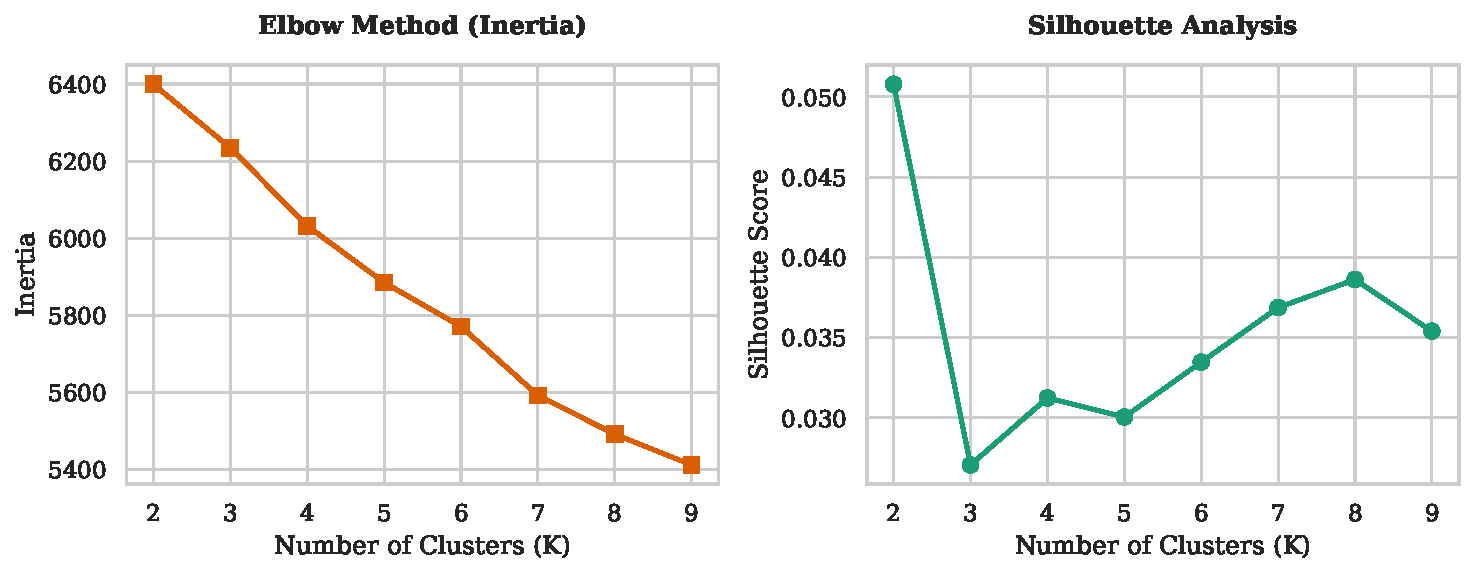
\includegraphics[width=0.9\textwidth]{Figures/kmeans_evaluation.pdf}
    \caption{Evaluation of k-Means Number of Clusters.}
    \label{fig:k_means}
\end{figure}

\begin{figure}[htbp]
    \centering
    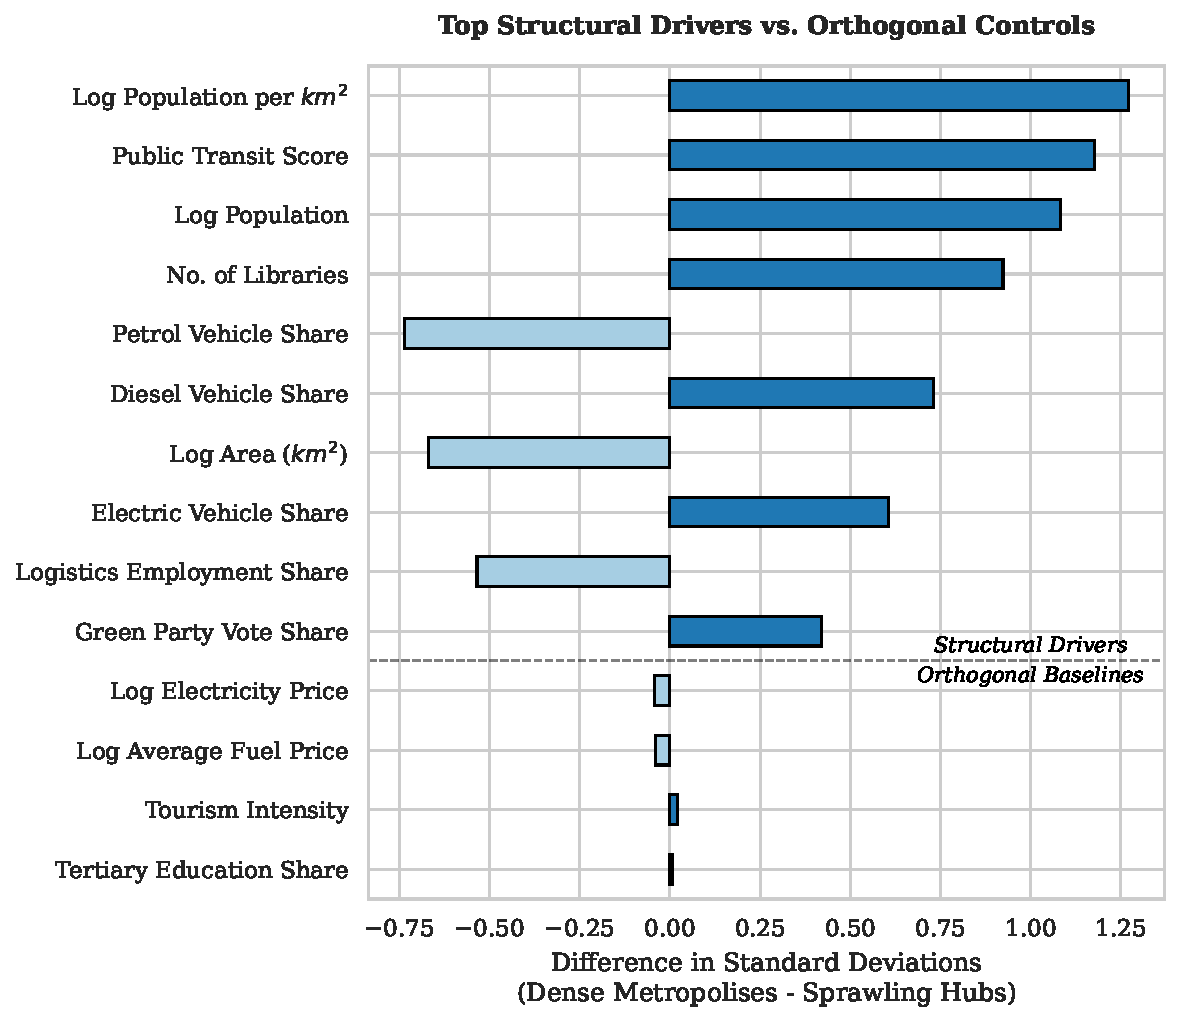
\includegraphics[width=0.9\textwidth]{Figures/cluster_differences.pdf}
    \caption{Differences between the two clusters.}
    \label{fig:cluster differences}
\end{figure}

% Figure 1: The visual summary of the Global ATT for immediate impact.
\begin{figure}[htbp]
    \centering
    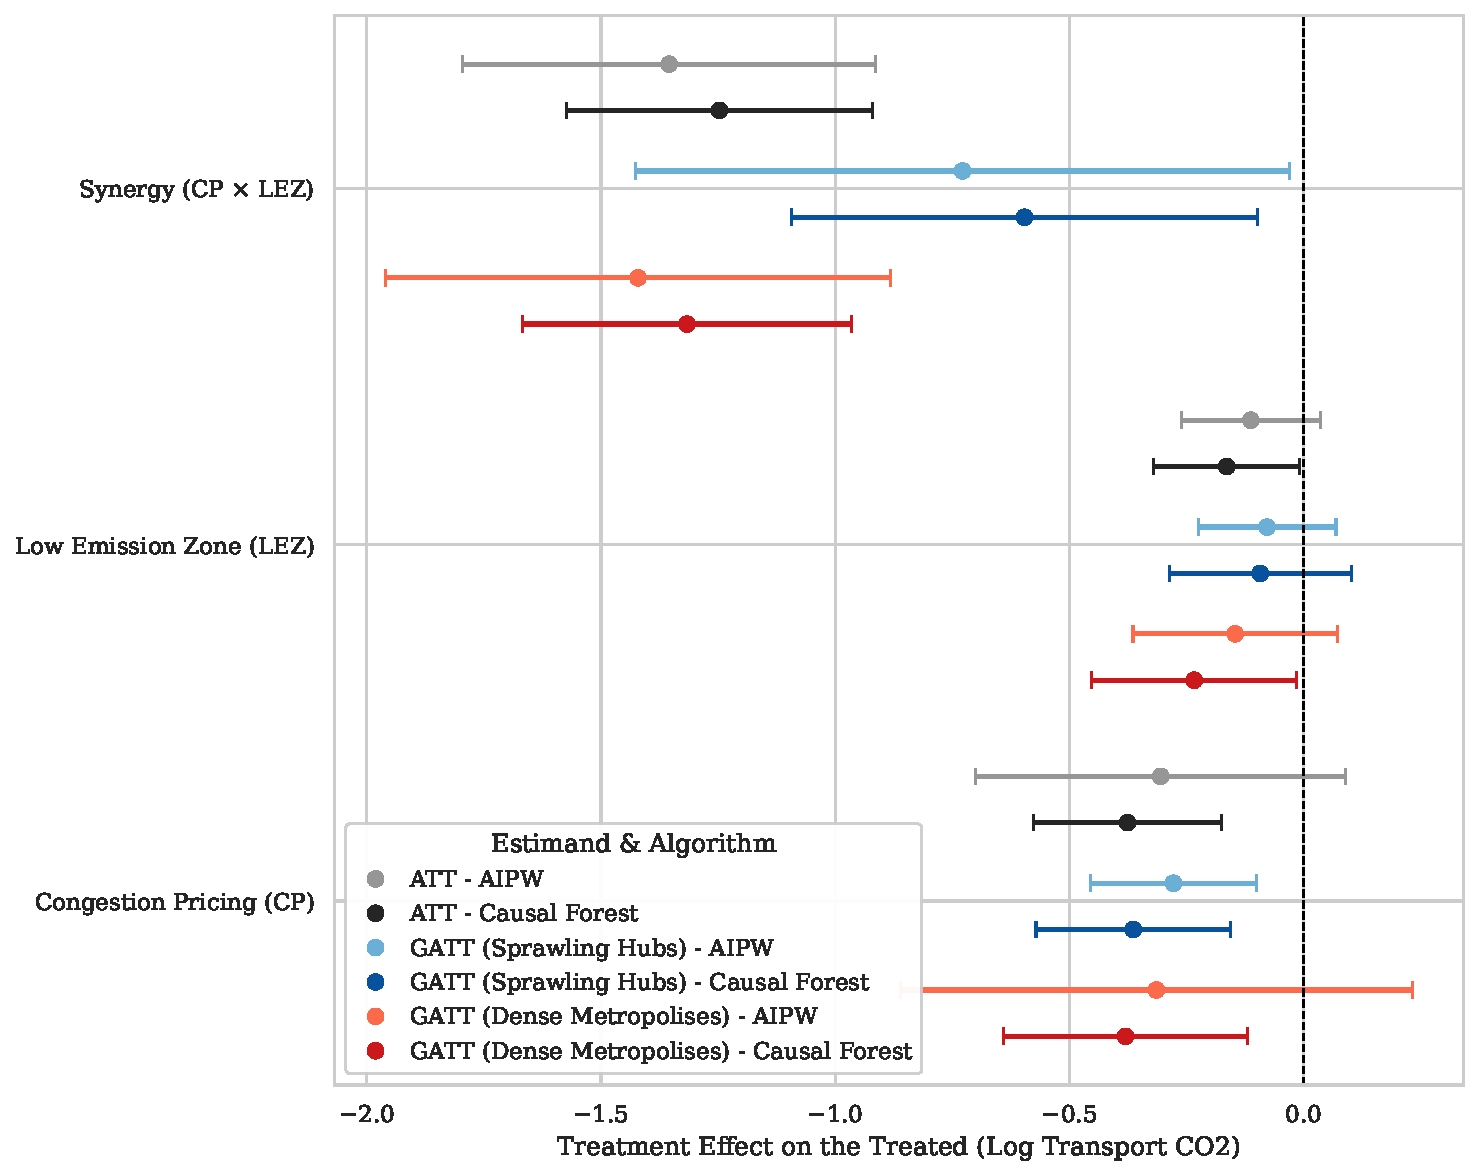
\includegraphics[width=0.9\textwidth]{Figures/forest_plot_att_gatt.pdf}
    \caption{Policy Efficacy by Algorithm (95\% CI)}
    \label{fig:forest_plot_att}
\end{figure}

\begin{figure}[htbp]
    \centering
    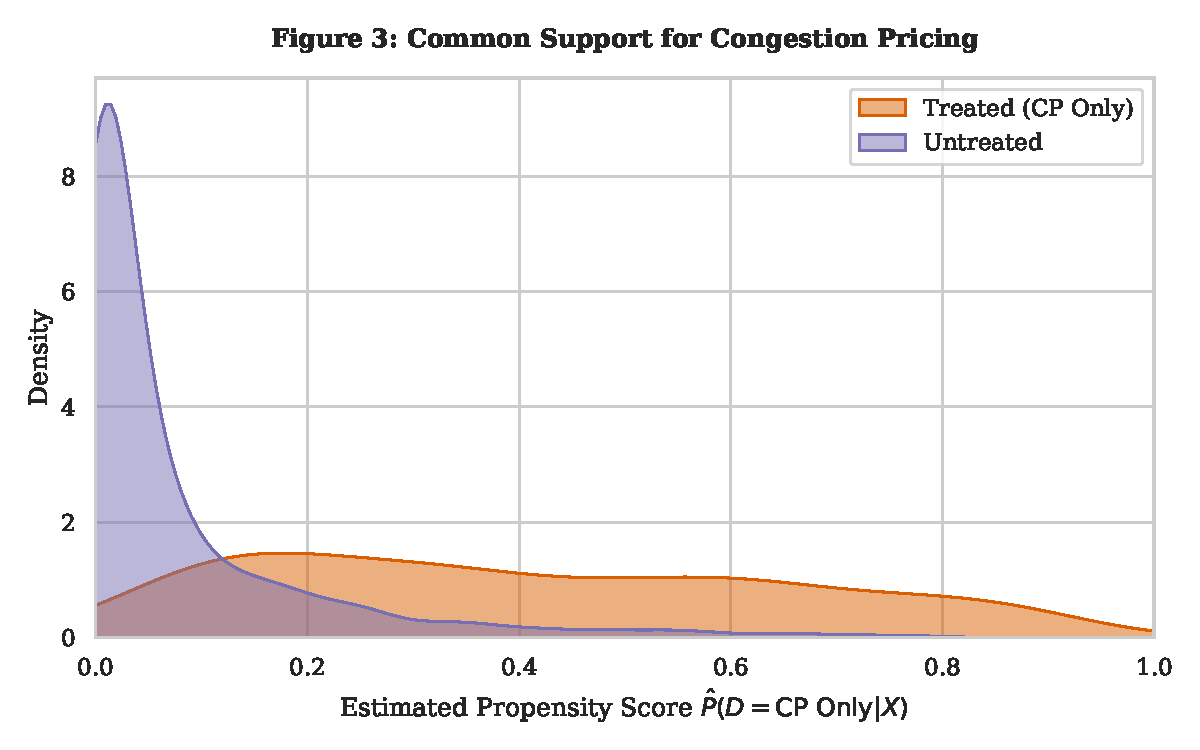
\includegraphics[width=0.8\textwidth]{Figures/overlap_density.pdf}
    \caption{Common Support for Congestion Pricing}
    \label{fig:overlap_density}
\end{figure}

% Positivity Trimming Graph (Ensure the line remains stable across thresholds).
\begin{figure}[htbp]
    \centering
    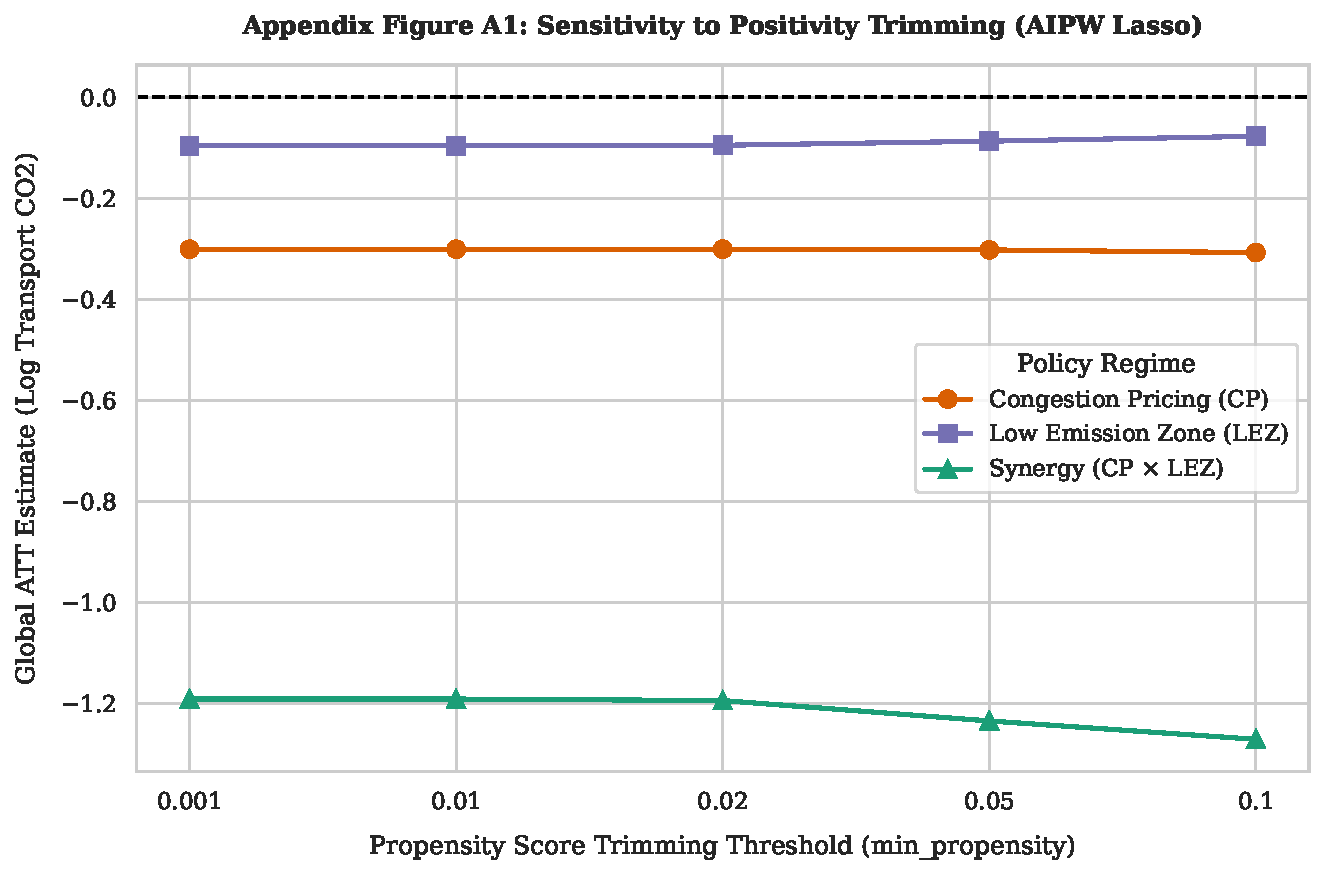
\includegraphics[width=0.8\textwidth]{Figures/appendix_overlap_sensitivity.pdf}
    \caption{Sensitivity to Positivity Trimming}
    \label{fig:appendix_overlap_sensitivity}
\end{figure}

 \begin{table}[htbp]
\centering
\caption{Falsification Tests: Estimated Effects on Placebo Outcomes (Global ATT)}
\label{tab:placebo_tests}
\begin{tabular}{lccc}
\toprule
Decoy Outcome & Congestion Pricing (CP) & Low Emission Zone (LEZ) & Synergy (CP $\times$ LEZ) \\
\midrule
\multicolumn{4}{l}{\textbf{Panel A: AIPW (Lasso)}} \\
\midrule
No. of Libraries & $-0.0370$ ($p=0.184$) & $0.0606$ ($p=0.216$) & $0.1269$ ($p=0.571$) \\
Streetlight Density & $0.8913$ ($p=0.470$) & $-0.8973$ ($p=0.215$) & $-0.4583$ ($p=0.861$) \\
No. of Fountains & $-0.3113$ ($p=0.383$) & $-0.1112$ ($p=0.652$) & $-0.3178$ ($p=0.470$) \\
No. of benches pc & $0.0205$ ($p=0.830$) & $-0.4880^{***}$ ($p=0.000$) & $-0.1854$ ($p=0.234$) \\
\midrule
\multicolumn{4}{l}{\textbf{Panel B: Causal Forest}} \\
\midrule
No. of Libraries & $-0.0695^{*}$ ($p=0.072$) & $0.1027^{**}$ ($p=0.032$) & $0.0047$ ($p=0.953$) \\
Streetlight Density & $1.7757^{**}$ ($p=0.038$) & $0.0723$ ($p=0.921$) & $0.8840$ ($p=0.438$) \\
No. of Fountains & $-0.5208$ ($p=0.106$) & $-0.3118$ ($p=0.166$) & $-0.3605$ ($p=0.428$) \\
No. of benches pc & $-0.0289$ ($p=0.835$) & $-0.5272^{***}$ ($p=0.000$) & $-0.3600^{**}$ ($p=0.031$) \\
\bottomrule
\end{tabular}
\raggedright \footnotesize \textit{Notes:} $p$-values in parentheses. $^{*}$ $p < 0.10$, $^{**}$ $p < 0.05$, $^{***}$ $p < 0.01$.
\end{table}


\clearpage
\section*{Declaration of Authorship}

I confirm that this report is based on my own work. In preparing this report, I have not received any help from another human nor have I discussed any aspects of the empirical project with others.

\vspace{10mm} %10mm vertical space


\includegraphics[width=0.2\textwidth]{Ferdinand_Unterschrift.PNG}

Ferdinand Loser

\end{document}